\chapter{Implementation}
\begin{quote}
    In this chapter, we give a comprehensive overview of the implementation of the CLMR model. We provide a PyTorch \cite{pytorch2019} implementation for both CLMR and CPC. The code implementation can be found on GitHub.\footnote{\url{https://github.com/spijkervet/CLMR}}
\end{quote}


\section{CLMR}
The CLMR model extends the vision contrastive learning framework, SimCLR \cite{chen_simple_2020}. We implemented their paper in PyTorch and ran extensive experiments to ensure it met the original paper's results.
We provide the code on GitHub as well.
\footnote{With 250+ stars and 50+ forks, our code has grown into one of the most popular PyTorch implementations of this framework: \url{https://github.com/spijkervet/SimCLR}}
\footnote{After we published the code, the original author, Ting Chen, also published their implementation in TensorFlow. We are cited as one of the PyTorch implementations in their work \url{https://github.com/google-research/SimCLR}}

\subsection{Optimising Audio Transformations}
The data augmentation pipeline consists of functions from the following code libraries:
\begin{verbatim}
    essentia
    torchaudio
    librosa
    sox
    wavaugment
\end{verbatim}
We use large mini-batch sizes for training, and while every mini-batch must contain randomly augmented examples, it is of significant importance to optimise the runtime of a parallelised augmentation pipeline.
Since audio transformations are CPU-intensive operations, most libraries have optimised their code by creating an interface between Python and languages that map their code more efficiently to machine instructions, e.g., the C language, to avoid a bottleneck on these augmentations.
\footnote{Python is an interpreted language, which makes it slower than machine code because making interpretations of instructions takes longer than executing machine instructions directly.}
However, both pitch-shifting and reverberation have not yet been fully optimised for Python. The code implementation of WavAugment provides a Python - C++ interface to interact with all audio effects in the sox library from within Python \cite{wavaugment2020}.
We use this implementation to significantly speed up pitch-shift and reverberation transformations in our augmentation pipeline.

\subsection{GPU Parallelisation}
PyTorch provides two interfaces to parallelise training on GPU's.
This can be used to either scale up the model, i.e., by increasing the number of parameters or by increasing the mini-batch size, or to speed up training.
The `DataParallel' (DP) module parallelises the data across multiple GPU's on a single node, while `DistributedDataParallel' (DDP) distributes it over multiple GPU's across multiple nodes.
We use either DP or DDP to speed up training or to increase the mini-batch size.
The maximum available hardware provided for this thesis was a a single $4\times \text{Titan RTX}$ node with 96 gigabytes of GDDR6 memory.
\footnote{We would like to thank SURFsara for providing the GPU nodes on the lisa system.}
This allowed us to train our largest model with a mini-batch size of 456. We leave further model scaling for future work.

As described earlier, batch normalisation is used in the convolution block to stabalise training, especially for larger mini-batch sizes \ref{tab:conv_block}.
Since information about batch statistics could leak to the learning objective, we utilise global batch normalisation.
It aggregates the operation from the devices to a single GPU device, and subsequently distributes the results to the other devices.

For multi-node training using DDP, the losses from all devices need to be aggregated in a similar way to avoid leakage of mini-batch information, i.e., the positive, anchor and negative samples. We used a gathering operation in PyTorch to aggregate losses from the NT-Xent function from all GPU devices.

\subsection{Encoder}
Our code implementation for CLMR allows for any encoder to be attached.
In this thesis, we implemented the SampleCNN encoder in PyTorch as our feature extractor.
The SampleCNN encoder consists of 11 convolution blocks, with varying kernel sizes and strides depending on the sample rate of the input audio. Its full structure is already shown in Table \ref{tab:samplecnn_model}.
With an input audio length of $±2.7$ seconds, the configuration of the kernel size and strides are listed in Table \ref{tab:samplecnn_config}.
The number of channels in the convolution block for each configuration is kept constant: $[128, 128, 128, 128, 256, 256, 256 , 256, 256, 512, 512]$.

\begin{table}
    \centering
        \begin{tabular}{lllll}\toprule
        Sample rate (Hz) & Audio length & Kernel size / Stride & \\\midrule
        22050 & $59049$  & $[3, 3, 3, 3, 3, 3, 3, 3, 3]$ \\
        16000 & $43470$ & $[3, 3, 3, 3, 3, 3, 5, 2, 2]$ \\
        8000 & $20736$ & $[3, 3, 3, 2, 2, 4, 4, 2, 2]$ \\                       
        \bottomrule
        \end{tabular}
    \caption{Kernel size and strides for different sample rates}
    \label{tab:samplecnn_config}
\end{table}

\section{Contrastive Predictive Coding}
We refer the reader to Figure \ref{fig:cpc_model} for a schematic overview of CPC, which puts the following details in a better perspective.

We adjusted the original CPC encoder $g_{\mathrm{enc}}$ to a structure similar to that of SampleCNN's to compare the effectiveness of this contrastive learning strategy more directly with CLMR and supervised benchmarks.
The encoder $g_{\mathrm{enc}}$ consists of 7 layers with 512 filters each, and filter sizes $[10, 6, 4, 4, 4, 2, 2]$ and strides $[5, 3, 2, 2, 2, 2, 2]$.
This results in a downsampling factor of $490$, which yields a feature vector for every $\approx$ 5~ms of audio for an input of 59\,049 samples.
Instead of relying on max-pooling, the filter sizes and strides are adjusted accordingly to parameterise and facilitate downsampling.
We also increased the number of prediction steps $k$ to 20, effectively asking the network to predict 100~ms of audio into the future.
The mini-batch size, i.e., the number of training examples the model is exposed to at once, is set to 64 from which 15 negative samples in the contrastive loss are drawn.

\section{Optimisation}
For asymmetric, non-linear activation functions like ReLU, it has been demonstrated that initialising the model parameters using Kaiming initialisation allows for faster model convergence \cite{he2015delving}.
We employ Kaiming initialisation for both CLMR and CPC. The following optimisers are used for pre-training. For smaller batch sizes, i.e., $< 96$, we use the Adam optimiser with a learning rate of $0.0003$ and $\beta_1 = 0.9$ and $\beta_2 = 0.999$. 
For larger batch sizes, i.e., $\geq 96$, we use the LARS optimiser with  square root learning rate scaling shown in Equation \ref{eq:sqrt_lr}, a cosine annealing schedule \ref{fig:cosine_annealing_lr} for the learning rate and a weight decay of $10^{-6}$.
This has shown to benefit contrastive learning when using a mini-batch size $\leq 4096$ \cite{chen_simple_2020}.

\begin{marginfigure}
    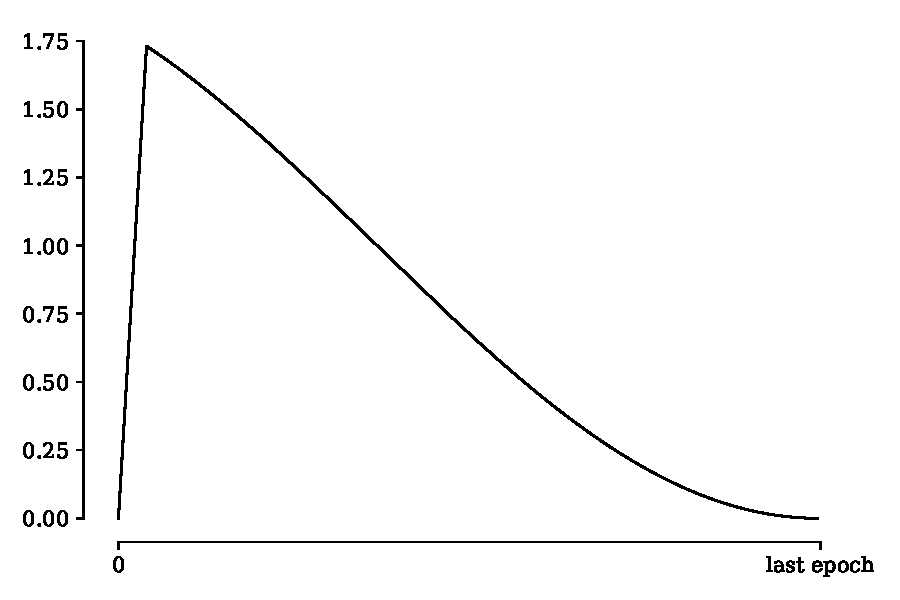
\includegraphics[width=\textwidth]{figs/cosine_annealing_schedule.pdf}
    \caption{Learning rate schedule: a warm-up is performed before the learning rate is adjusted using a cosine annealing schedule. In this example, the learning rate linearly scales to 1.75 before decreasing back to near-zero at the last epoch.}
    \label{fig:cosine_annealing_lr}
\end{marginfigure}

\begin{equation}
    \label{eq:sqrt_lr}
    Learning Rate = 0.075 * \sqrt{Batch Size}
\end{equation}

For linear evaluation, we use the Adam optimiser with a learning rate of $0.0003$ and a weight decay of $10^{-6}$. Backpropagation is only done in the fine-tune head, i.e., it only optimises the linear layer or MLP. The pre-trained encoder remains frozen in all evaluation procedures, for the full classification, efficient classification and transfer learning experiments.
We also employ an early stopping mechanism when the validation scores do not improve for 3 epochs. \footnote{Early stopping stops training on the larger train set, when it has shown to generalise on a smaller validation set.}